\chapter{Conclusiones y Perspectivas}
\section{Conclusiones}
En el presente estudio se encontraron las condiciones necesarias para extraer ion litio presente a bajas concentraciones en medios acuosos usando una membrana polimérica de inclusión de CTA. Los extractantes mas apropiados fueron LIX-54-100 y Cyanex~923 en una relación molar 2.15:1. La membrana no requiere la adición de un plastificante en su formulación. El Cyanex~923 tiene la función doble como extractante y plastificante. El sistema presenta buena selectividad frente a los cationes alcalinos sodio y potasio pero los cationes divalentes no son excluidos eficientemente por la membrana. La metodología propuesta fue exitosamente aplicada a la extracción del ion litio presente en muestras de mar. Para esto es necesario retirar por precipitación los cationes divalentes. La propuesta que se hizo fue elevar el pH del medio con hidróxido de sodio, centrifugar la suspensión, añadir una pequeña cantidad de fosfato de amonio a la fase líquida y centrifugar de nuevo para retirar los sólidos suspendidos. El proceso de recobro de ion litio a partir de agua de mar, haciendo uso del protocolo propuesto en este trabajo se esquematiza en la Figura \ref{fig:diagrama}.

{\floatstyle{boxed}
\restylefloat{figure}
\begin{figure}[h]
    \centering
    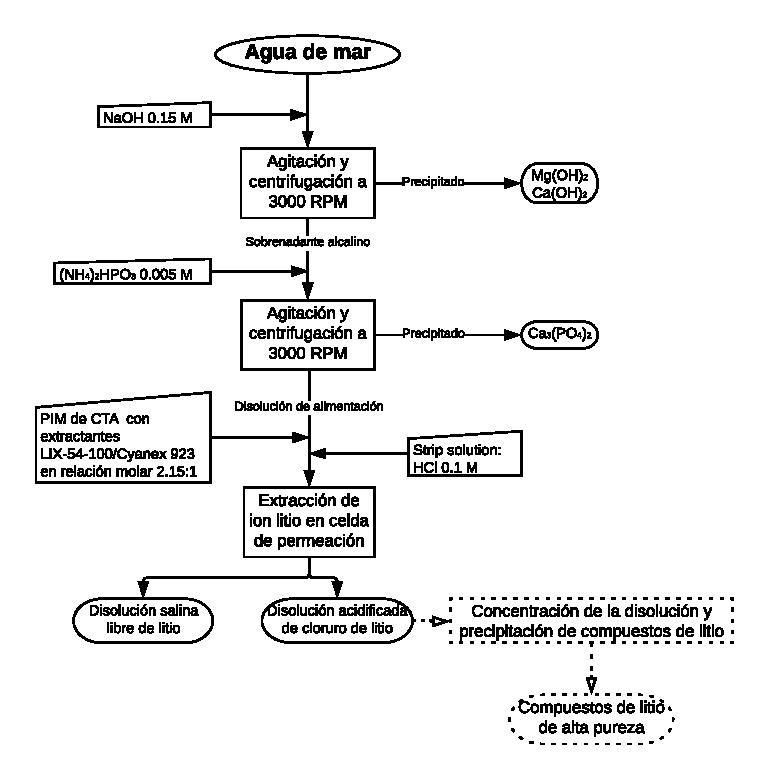
\includegraphics[width = 0.8\textwidth]{chap6/DiagramaProcesoLitioTesis.pdf}
    \caption[Proceso de recobro de ion litio a partir de agua de mar.]{Proceso de recobro de ion litio a partir de agua de mar. La sección del diagrama en línea discontinua son los pasos que no fueron considerados en el presente trabajo.}
    \label{fig:diagrama}
\end{figure}}

La reutilización de las disoluciones de recuperación permiten concentrar al ion litio. Esto fue posible con las disoluciones ideales en las que el ion litio es el único catión metálico presente y con las muestras de agua de mar que contienen excesos molares de iones sodio y potasio de 18000 y 400, respectivamente frente al ion litio. Cuando se concentra el ion litio presente en agua de mar es necesario restaurar el gradiente protónico a través de la membrana al final de cada ciclo para que el transporte pueda ocurrir. No se evaluó la opción de mantener constante el pH de la disolución de recuperación haciendo uso de sustancias amortiguadoras de pH porque se deseó mantener la matriz de las disoluciones tan simple como fuese posible. La selectividad y la eficiencia de la membrana se deterioran con cada ciclo de uso.

La membrana puede ser reutilizada pero tras cada ciclo de uso se pierde eficiencia en el proceso. La membrana tiene una estabilidad regular al conservar solo el 60\% de su capacidad tras diez ciclos de uso de seis horas. El deterioro de la membrana es más marcado cuando se usa agua de mar como disolución de alimentación. Cuando se compara agua de mar sintética simplificada y agua de mar natural el comportamiento del sistema es prácticamente el mismo. 

El coeficiente de permeabilidad de la membrana frente al ion litio, calculado con la Ecuación \ref{eq:coefPerm}, es 2.1 $\times10^{-5}$ m s$^{-1}$. La selectividad del sistema luego de retirar los cationes divalentes del medio es $\ce{Li+}>>\ce{Na+}>\ce{K}$. Los factores de separación en respecto al sodio y al potasio en agua de mar alcanzan valores de hasta 40 y 110, respectivamente. En los factores de separación los valores más altos representan un sistema más selectivo.

Respecto a la disolución de alimentación, se encontró que para que el transporte de ion litio sea posible usando el sistema propuesto, es necesario que la disolución de alimentación sea alcalina. Debido a la naturaleza del algoritmo simplex modificado escogido para optimizar el sistema, no se determinó el valor mínimo de pH necesario para que el transporte de ion litio ocurra, pero este valor debe encontrarse por encima del pKa del LIX-54-100. El pKa del LIX-54-100 debe ser similar al del benzoilacetona (9.61 \citep{Witt2017}). 

Se ha dado cumplimiento al objetivo general y a los objetivos específicos del proyecto. La hipótesis inicial del trabajo ha sido confirmada. El método propuesto podría eventualmente ser adaptado a una escala mayor a la del laboratorio, pero antes de eso deben hacerse consideraciones cuidadosas sobre el posible impacto ambiental y social que puede conllevar la extracción de ion litio a partir de agua de mar. Parece razonable suponer que el impacto a los ecosistemas marinos a causa de la disminución en la concentración de ion litio puede ser pequeño debido al inmenso volumen de agua contenida en los océanos. La extracción del 0.5\% del ion litio presente en los océanos representa una cantidad de litio mucho mayor a la que se ha extraído en toda la historia de la humanidad.

La ecuación empírica propuesta para modelar los perfiles de transporte presenta un excelente ajuste a los datos experimentales y ha resultado de gran ayuda para estudiar la evolución del sistema. De manera similar, el método planteado en la Sección \ref{app:ParedesMethod} para determinar la significancia del efecto de variables explicatorias en un diseño factorial fraccionado ha arrojado resultados muy similares a los que pueden obtenerse con el método gráfico que deriva del dia\-grama de Daniel o con el método de Lenth para determinar la significancia de dichos efectos. Esta metodología presenta algunas similitudes con el algoritmo \ac{NIPALS} que optimiza el número de componentes principales necesarios para describir adecuadamente un conjunto de datos tras la transformación lineal de un \ac{PCA} \citep{Wehrens2011}. Determinar la significancia por este método puede presentar una ventaja sobre el análisis gráfico con los diagramas de Daniel de que no se requiere la asunción \textit{escasez} de efecto.


El paquete \verb|transmem| facilitó significativamente el tratamiento de los datos producidos. Las repre\-sentaciones gráficas que genera son claras, consistentes y estéticas. Tras unos pocos meses luego de su aceptación en el repositorio oficial \ac{CRAN} \citep{transmem}, el paquete ya cuenta con más de 2000 descargas. Se trabajará en su difusión para que sea de utilidad para un mayor número de grupos de investigación que trabajan en el transporte a través de membranas.

\section{Perspectivas}
En el presente trabajo la separación del ion litio no concluyó en la obtención final de un compuesto sólido sino que se obtuvo una disolución en la cual la relación molar de ion litio respecto a otros cationes metálicos es mucho mayor a la originalmente presentada en el agua de mar. La concentración de ion litio en este medio sigue siendo demasiado pequeña como para producir un compuesto de ion litio con un alto nivel de pureza por alguna técnica como precipitación \citep{Nishihama2011}. La obtención de un reactivo con valor comercial a un buen nivel de pureza a partir de la disolución resultante del presente protocolo puede ser el paso a seguir si se desea continuar con el desarrollo del método de extracción propuesto.

Múltiples mejoras pueden ser implementadas al proceso con el fin de proponer una vía más plausible hacia la aplicación del método en el mundo real.

Respecto a los iones divalentes del medio, se ha reportado que el uso de hidróxido de sodio como agente precipitante para la remoción de magnesio presenta conflictos en la posterior separación de fases porque el precipitado que se forma tiene características coloidales \citep{An2012}. El protocolo propuesto en este trabajo involucra hidróxido de sodio e incluye pasos de maduración de precipitado con agitación vigorosa y centrifugación a 3000 \ac{RPM} durante cinco minutos. La separación de fases fue lograda efectivamente y el precipitado formado tiene una excelente consistencia que permite voltear deliberadamente las celdas de centrifugación para recuperar las aguas madres. Considerando las afirmaciones de \citet{An2012}, es probable que este comportamiento tan ideal no sea tan fácil de lograr en escala de planta piloto o planta de producción. 

Una alternativa que valdría la pena probar para remover el magnesio y el calcio puede ser el método de electrólisis de membrana propuesto por \citet{Diaz2019}. Esta puede ser una excelente alternativa para retirar estos cationes del agua de mar sin aumentar la concentración de iones sodio en el medio. Otra ventaja de este procedimiento es que los hidróxidos de calcio y magnesio se obtienen individualmente como precipitados de alto nivel de pureza y podría ser posible su comercialización, con lo que la viabilidad económica del proyecto en conjunto podría ser mayor. Este proceso de electrólisis de membrana puede proveer al medio de la alcalinidad requerida para el proceso de extracción de ion litio usando el protocolo del presente trabajo. La membrana que requiere el método de \citet{Diaz2019} es selectiva a aniones y transporta iones cloruro para mantener la electroneutralidad en ambos compartimientos de la celda. La membrana además evita que los protones generados en el compartimiento anódico neutralicen la disolución y se residuelvan los hidróxidos que se están retirando. La membrana selectiva a aniones podría ser innecesaria si se usa un ánodo de plata, sobre el cual podría depositarse cloruro de plata a medida que en el cátodo se presenta la evolución de hidrógeno con la respectiva formación de iones hidroxilo como consecuencia de la reducción del agua. El electrodo de plata queda recubierto de cloruro de plata con lo que en algún momento quedaría inutilizable, pero puede ser regenerado a través de la inversión del potencial aplicado (en una disolución salina) para reducir la plata del cloruro de plata.

Por otro lado, para concentrar el licor de ion litio que se obtiene como disolución de recuperación, puede probarse la ósmosis directa usando membranas de \ac{CTA} que ha sido aplicada por \citet{Li2018} para retirar parte importante del disolvente y aumentar la concentración de ion litio en una salmuera de un lago salado. Esta técnica no produce subproductos indeseables y el gasto energético es mínimo dado que contrario a la ósmosis inversa, la fuerza motriz en este caso es el potencial osmótico propio de las disoluciones. Como disolución de arrastre podría usarse el agua de mar que ya fue utilizada en el proceso de extracción de ion litio. 

Durante los experimentos de concentración de ion litio de agua de mar, la celda de transporte se dejó en laboratorio durante una semana y se observó una disminución progresiva del volumen de la disolución de recuperación con un aumento de similar proporción en el volumen de la disolución de alimentación. No se determinó si el ion litio presente en la disolución de recuperación había aumentado su concentración, pero es probable que un proceso de ósmosis directa haya tenido lugar ya que membranas de \ac{CTA} han demostrado ser de utilidad para este tipo de procedimientos \citep{Li2018}.

Un trabajo futuro podría incorporar un potencial eléctrico como fuerza motriz para el transporte de ion litio a través de la \ac{PIM}. Los métodos electroquímicos acoplados a membranas selectivas son actualmente muy estudiados y han sido exitosamente aplicados a la extracción de ion litio a partir de agua de mar \citep{LIU2019}. Adaptar este enfoque a la PIM propuesta en esta tesis podría generar electrodialisis selectiva de membrana. Esta combinación de técnicas ha sido empleada en distintas ocasiones para mejorar el transporte de diversas especies a través de PIMs \citep{Kaya2016, See2013} pero aún no ha sido aplicada al transporte de ion litio a través de estas membranas.

El impacto ambiental de la fabricación de las membranas podría disminuirse si se evalúa la preparación de las PIMs usando el proceso libre de disolventes reportado por \citet{Vera2019}. Al no usar disolventes orgánicos clorados, la emisión de vapores perjudiciales para la atmósfera es anulada. Esto requiere que se caractericen térmicamente los extractantes y que se reemplace el polímero base por uno con punto de fusión más bajo \citet{Vera2019}.

La estabilidad y la permeabilidad de la membrana frente a iones litio podría incrementarse significativamente si se incursiona en el uso de polímeros base entrecruzables para producir PIMs de \textit{nueva generación} \citep{OBRYAN2017}.

Finalmente, un nuevo trabajo de tesis relacionado con la extracción de ion litio usando PIMs podría involucrar el uso de líquidos iónicos similares a los reportados por \citet{ZANTE2019} o por \citet{Shi2020}. El desempeño de esta nueva membrana puede ser comparado con el de las membranas reportadas en el presente trabajo. Las perspectivas propuestas en párrafos anteriores podrían ser probadas en la membrana que resulte más apta tras hacer la comparación. El trabajo interdisciplinar involucraría la síntesis de los líquidos iónicos y el estudio del sistema electroquímico para la extracción.
\clearpage
\ChapBib{chap6/conclusions}